\documentclass{ieeetj}
\usepackage{cite}
\usepackage{amsmath,amssymb,amsfonts}
\usepackage{graphicx,color}
\usepackage{textcomp}
\usepackage{xcolor}
\usepackage{hyperref}
\hypersetup{hidelinks=true}
\usepackage{booktabs}
\usepackage{url}
\setlength{\emergencystretch}{2em}

\AtBeginDocument{%
  \definecolor{tmlcncolor}{cmyk}{0.93,0.59,0.15,0.02}%
  \definecolor{NavyBlue}{RGB}{0,86,125}}

\def\OJlogo{\vspace{-4pt}$<$Society logo(s) and publication title will appear here.$>$}
\def\seclogo{\vspace{10pt}$<$Society logo(s) and publication title will appear here.$>$}

\def\authorrefmark#1{\ensuremath{^{\textbf{#1}}}}

\renewcommand{\thetable}{S\arabic{table}}
\renewcommand{\thefigure}{S\arabic{figure}}
\makeatletter
\renewcommand{\@biblabel}[1]{[S#1]}
\renewcommand{\citeform}[1]{S#1}
\makeatother

\begin{document}
\receiveddate{XX Month, XXXX}
\reviseddate{XX Month, XXXX}
\accepteddate{XX Month, XXXX}
\publisheddate{XX Month, XXXX}
\currentdate{XX Month, XXXX}
\doiinfo{XXXX.2026.1234567}

\markboth{}{Franklin}

\title{Supplemental Material for: Adaptive Phase-Switching for Communication-Efficient Federated LoRA Fine-Tuning}

\author{Jerry Adams Franklin\authorrefmark{1}}
\affil{Independent Researcher, Fairport, NY 14450 USA}
\corresp{Corresponding author: Jerry Adams Franklin (email: jerry.adamsf@gmail.com). ORCID: 0009-0006-8470-8349.}

\begin{abstract}
This supplemental material accompanies the main paper. It provides
hyperparameter details, per-seed results for every configuration reported in
the main paper, paired significance tests with a multiplicity correction, a
reproducibility checklist, cross-backend verification of the full run corpus,
the downstream zero-shot accuracy figure, and the mechanics of disabling the
ReverseAdaptive switch. Tables and figures in this document carry an S prefix
and reference numbers in square brackets carry an S prefix, so that
cross-references to the main paper are unambiguous. Cross-references to the
main paper use fixed table and section numbers from the compiled manuscript.
\end{abstract}

\begin{IEEEkeywords}
Communication efficiency, federated learning, large language models, low-rank adaptation, parameter-efficient fine-tuning.
\end{IEEEkeywords}

\maketitle
\appendices

\section{Hyperparameter Details}
\label{app:hyper}
All experiments use AdamW \cite{loshchilov2019decoupled} with learning rate $10^{-4}$, $\beta_1{=}0.9$, $\beta_2{=}0.999$. No learning rate schedule is applied. Gradients are clipped to a maximum $\ell_2$ norm of 1.0 at every optimizer step. Maximum sequence length is 256 tokens. See Table~1 of the main paper for the complete configuration including ReverseAdaptive defaults.

\section{Per-Seed Full Results}
\label{app:perseed}
Tables in this appendix are labeled with their corpus. Per-seed results backing a method comparison use the CUDA corpus, matching the main results tables; per-seed results documenting partition sensitivity retain the larger MPS seed set, where five seeds at $\alpha{=}0.1$ provide better evidence than three.

At $\alpha{=}0.5$, mean final loss is statistically indistinguishable from IID for every method in the released analysis CSVs, with differences of 0.001 to 0.007 against per-seed standard deviations near 0.02 over three seeds. Heterogeneity manifests instead as sensitivity to the partition draw: seed-to-seed standard deviation rises by roughly an order of magnitude, from $0.5$ to $1.6 \times 10^{-3}$ under IID in Table~\ref{tab:b1} to $18$ to $25 \times 10^{-3}$ at $\alpha{=}0.5$ across the methods in the released CSVs, which is also why the per-seed spread at $\alpha{=}0.1$ in Table~\ref{tab:b2} is wide.

\begin{table*}[t]
\caption{Per-seed TinyLlama-1.1B IID results, CUDA corpus, backing Table~2 of the main paper. Communication is deterministic across seeds. $\dagger$ For Two-Phase the column shows the predetermined phase boundary $K$, not an adaptive switch event; for FFA-LoRA, $A$ is frozen from initialization; for ReverseAdaptive it shows the round at which the plateau signal triggered.}
\label{tab:b1}
\begin{center}
\small
\setlength{\tabcolsep}{6pt}
\begin{tabular}{llccc}
\toprule
Method & Seed & Final loss & Total MB & Switch / boundary$^\dagger$ \\
\midrule
FLoRA & 42 & 1.261408 & 2578.13 & -- \\
FLoRA & 123 & 1.260479 & 2578.13 & -- \\
FLoRA & 456 & 1.260500 & 2578.13 & -- \\
FedIT & 42 & 1.260767 & 2578.13 & -- \\
FedIT & 123 & 1.258420 & 2578.13 & -- \\
FedIT & 456 & 1.261503 & 2578.13 & -- \\
Two-Phase $K{=}8$ & 42 & 1.271276 & 1863.13 & $K{=}8^\dagger$ \\
Two-Phase $K{=}8$ & 123 & 1.270130 & 1863.13 & $K{=}8^\dagger$ \\
Two-Phase $K{=}8$ & 456 & 1.270237 & 1863.13 & $K{=}8^\dagger$ \\
ReverseAdaptive ($\tau{=}0.01$) & 42 & 1.275514 & 1533.13 & 6 \\
ReverseAdaptive ($\tau{=}0.01$) & 123 & 1.274610 & 1533.13 & 6 \\
ReverseAdaptive ($\tau{=}0.01$) & 456 & 1.274481 & 1533.13 & 6 \\
FFA-LoRA & 42 & 1.303975 & \phantom{0}983.13 & init$^\dagger$ \\
FFA-LoRA & 123 & 1.301738 & \phantom{0}983.13 & init$^\dagger$ \\
FFA-LoRA & 456 & 1.303628 & \phantom{0}983.13 & init$^\dagger$ \\
\bottomrule
\end{tabular}
\end{center}
\end{table*}

\begin{table*}[t]
\caption{Non-IID results, MPS corpus, five seeds at $\alpha{=}0.1$. This table documents partition sensitivity rather than comparing methods, so the larger MPS seed set is retained; Table~\ref{tab:b1} follows the CUDA corpus because it backs a method comparison. Seeds 42 and 1000 at $\alpha{=}0.1$ had 9 and 8 active clients due to empty Dirichlet partitions, which scales communication to $9/10$ and $8/10$ of the full value (1379.81 and 1226.50 MB against 1533.13). Cross-backend verification (Appendix~\ref{app:crossbackend}) covers seeds 42, 123, and 456; seeds 789 and 1000 were executed on MPS only.}
\label{tab:b2}
\begin{center}
\footnotesize
\setlength{\tabcolsep}{4pt}
\begin{tabular}{llcccc}
\toprule
Setting & Seed & Final loss & Total MB & Switch round & Active clients \\
\midrule
ReverseAdaptive, $\alpha{=}0.5$ & 42 & 1.285933 & 1533.13 & 6 & 10 \\
ReverseAdaptive, $\alpha{=}0.5$ & 123 & 1.282625 & 1533.13 & 6 & 10 \\
ReverseAdaptive, $\alpha{=}0.5$ & 456 & 1.252133 & 1533.13 & 6 & 10 \\
ReverseAdaptive, $\alpha{=}0.1$ & 42 & 1.268353 & 1379.81 & 6 & 9 \\
ReverseAdaptive, $\alpha{=}0.1$ & 123 & 1.288985 & 1533.13 & 6 & 10 \\
ReverseAdaptive, $\alpha{=}0.1$ & 456 & 1.348083 & 1533.13 & 6 & 10 \\
ReverseAdaptive, $\alpha{=}0.1$ & 789 & 1.259200 & 1533.13 & 6 & 10 \\
ReverseAdaptive, $\alpha{=}0.1$ & 1000 & 1.273046 & 1226.50 & 6 & 8 \\
\bottomrule
\end{tabular}
\end{center}
\end{table*}

\begin{table}[!t]
\caption{Per-seed LLaMA-3.2-3B IID results, MPS corpus, backing Table~7 of the main paper. ReverseAdaptive uses $\tau{=}0.01$. Communication is deterministic given the switch round; the three ReverseAdaptive seeds occupy three adjacent lattice points.}
\label{tab:b3}
\begin{center}
\small
\setlength{\tabcolsep}{5pt}
\begin{tabular}{llccc}
\toprule
Method & Seed & Final loss & Total MB & Switch \\
\midrule
FLoRA & 42 & 1.371683 & 2625.0 & -- \\
FLoRA & 123 & 1.373402 & 2625.0 & -- \\
FLoRA & 456 & 1.371998 & 2625.0 & -- \\
Two-Phase $K{=}8$ & 42 & 1.393776 & 1942.5 & $K{=}8$ \\
Two-Phase $K{=}8$ & 123 & 1.394877 & 1942.5 & $K{=}8$ \\
Two-Phase $K{=}8$ & 456 & 1.392772 & 1942.5 & $K{=}8$ \\
ReverseAdaptive & 42 & 1.393831 & 1837.5 & 8 \\
ReverseAdaptive & 123 & 1.390265 & 1942.5 & 9 \\
ReverseAdaptive & 456 & 1.397366 & 1732.5 & 7 \\
\bottomrule
\end{tabular}
\end{center}
\end{table}

\begin{table}[!t]
\caption{Per-seed TinyLlama-1.1B Dolly-15k IID results, CUDA corpus, backing Table~3 of the main paper. Held-out $\Delta$ is tuned minus base on the Dolly-15k held-out slice; more negative is better.}
\label{tab:b4}
\begin{center}
\small
\setlength{\tabcolsep}{5pt}
\begin{tabular}{llccc}
\toprule
Method & Seed & Final loss & Held-out $\Delta$ & Total MB \\
\midrule
FLoRA & 42 & 1.656762 & $-0.531848$ & 2578.13 \\
FLoRA & 123 & 1.652934 & $-0.533376$ & 2578.13 \\
FLoRA & 456 & 1.653426 & $-0.533664$ & 2578.13 \\
Two-Phase $K{=}8$ & 42 & 1.666616 & $-0.527571$ & 1863.13 \\
Two-Phase $K{=}8$ & 123 & 1.662685 & $-0.529113$ & 1863.13 \\
Two-Phase $K{=}8$ & 456 & 1.663475 & $-0.529410$ & 1863.13 \\
ReverseAdaptive & 42 & 1.671039 & $-0.526568$ & 1533.13 \\
ReverseAdaptive & 123 & 1.666995 & $-0.527418$ & 1533.13 \\
ReverseAdaptive & 456 & 1.667699 & $-0.526547$ & 1533.13 \\
\bottomrule
\end{tabular}
\end{center}
\end{table}



\section{Statistical Tests}
\label{app:stats}
Paired $t$-tests over three seeds on final-round training loss and on held-out instruction-following loss. TinyLlama-1.1B results use the CUDA corpus, matching Table~2 of the main paper; LLaMA-3.2-3B results use the MPS corpus.

With three seeds these tests have very low power, so effect sizes should be read alongside the $p$-values. No multiplicity correction is applied in the main results tables. Applying a Bonferroni correction across the six TinyLlama-1.1B Alpaca IID comparisons gives a threshold of $0.0083$, which the ReverseAdaptive versus Two-Phase $K{=}8$ comparison on held-out loss ($p = 0.026$) does not meet. That comparison is secondary under the frontier framing of Section~V of the main paper; the load-bearing comparison is ReverseAdaptive versus FFA-LoRA, which holds at $p < 10^{-3}$ on both metrics with a difference roughly twenty times the largest per-method standard deviation.

The LLaMA-3.2-3B comparison between ReverseAdaptive and Two-Phase $K{=}8$ has a 95\% confidence interval of $[-0.0114, 0.0114]$, which contains the $0.0043$ difference observed between the same methods at TinyLlama-1.1B. The test therefore cannot distinguish equivalence from a difference of the magnitude seen at the smaller scale.

\begin{table*}[t]
\caption{Paired $t$-tests, three seeds. TinyLlama-1.1B rows use the CUDA corpus; LLaMA-3.2-3B rows use MPS. Positive $\Delta$ indicates the first method has higher loss.}
\label{tab:d1}
\begin{center}
\footnotesize
\setlength{\tabcolsep}{4pt}
\begin{tabular}{lcccc}
\toprule
Comparison & $\Delta$ final loss & $p$ & $\Delta$ held-out & $p$ \\
\midrule
\multicolumn{5}{l}{\emph{TinyLlama-1.1B, Alpaca, IID}} \\
Two-Phase $K{=}8$ vs.\ FLoRA & $+0.0098$ & $4.2 \times 10^{-5}$ & $+0.0034$ & $7.9 \times 10^{-5}$ \\
ReverseAdaptive vs.\ FLoRA & $+0.0141$ & $1.1 \times 10^{-5}$ & $+0.0063$ & $6.2 \times 10^{-3}$ \\
ReverseAdaptive vs.\ Two-Phase $K{=}8$ & $+0.0043$ & $3.4 \times 10^{-4}$ & $+0.0029$ & $2.6 \times 10^{-2}$ \\
FFA-LoRA vs.\ ReverseAdaptive & $+0.0282$ & $4.4 \times 10^{-4}$ & $+0.0182$ & $3.8 \times 10^{-4}$ \\
FFA-LoRA vs.\ FLoRA & $+0.0423$ & $1.7 \times 10^{-4}$ & $+0.0245$ & $1.1 \times 10^{-4}$ \\
FedIT vs.\ FLoRA & $-0.0006$ & $0.588$ & $+0.0002$ & $0.425$ \\
\midrule
\multicolumn{5}{l}{\emph{TinyLlama-1.1B, Dolly-15k, IID}} \\
Two-Phase $K{=}8$ vs.\ FLoRA & $+0.0099$ & $7.8 \times 10^{-5}$ & $+0.0043$ & $2.4 \times 10^{-6}$ \\
ReverseAdaptive vs.\ FLoRA & $+0.0142$ & $2.5 \times 10^{-5}$ & $+0.0061$ & $7.6 \times 10^{-3}$ \\
\midrule
\multicolumn{5}{l}{\emph{LLaMA-3.2-3B, Alpaca, IID}} \\
Two-Phase $K{=}8$ vs.\ FLoRA & $+0.0214$ & $3.2 \times 10^{-4}$ & -- & -- \\
ReverseAdaptive vs.\ FLoRA & $+0.0215$ & $1.3 \times 10^{-2}$ & -- & -- \\
ReverseAdaptive vs.\ Two-Phase $K{=}8$ & $+0.000012$ & $0.997$ & -- & -- \\
\bottomrule
\end{tabular}
\end{center}
\end{table*}

\begin{figure*}[!t]
\begin{center}
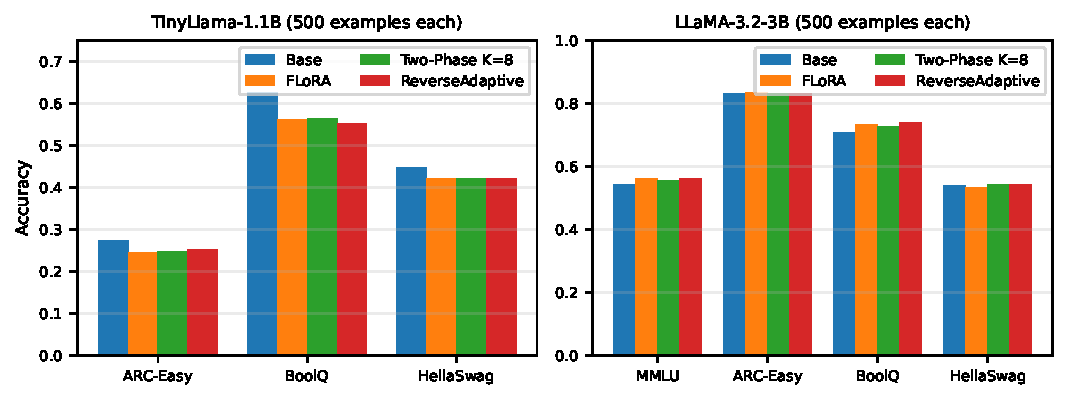
\includegraphics[width=\textwidth]{figures/fig4_downstream_accuracy.pdf}
\end{center}
\caption{Downstream zero-shot accuracy across two model scales (500 examples per benchmark). Left: TinyLlama-1.1B (seed 42 only; ARC-Easy, BoolQ, HellaSwag; MMLU omitted because base accuracy is at chance for 4-way multiple choice). Right: LLaMA-3.2-3B (mean across three seeds; MMLU, ARC-Easy, BoolQ, HellaSwag). Federated methods cluster within 1.0 percentage points at TinyLlama-1.1B, across the three informative benchmarks, and 0.5 percentage points at LLaMA-3.2-3B. TinyLlama accuracies are single-seed and from the MPS corpus; loss values elsewhere in the main paper for the same configurations are three-seed and from the CUDA corpus.}
\label{fig:supp_downstream}
\end{figure*}

\section{Reproducibility Checklist}
\label{app:repro}
\textbf{Code:} Full source code is publicly released, including all configuration YAML files, training scripts, evaluation scripts, and scripts to reproduce every figure and table from the analysis CSVs.

\textbf{Seeds:} The IID seeds are listed in Table~1 of the main paper. The $\alpha{=}0.1$ partition-sensitivity runs additionally use seeds 789 and 1000, which appear only in Table~\ref{tab:b2} of this supplement. Per-seed results are in Appendix~\ref{app:perseed}.

\textbf{Hardware:} The primary corpus of 34 runs was produced on a single Apple M4 Pro workstation with 48\,GB unified memory using the MPS backend, approximately 285 hours of compute, with no institutional cluster. Those runs were re-executed on commercially rented NVIDIA hardware, an RTX 4090 for TinyLlama-1.1B and an A100 40\,GB for LLaMA-3.2-3B; the comparison is in Appendix~\ref{app:crossbackend}. The Dolly-15k replication and the FFA-LoRA and FedIT baselines were produced on the rented hardware only.

\textbf{Data:} Alpaca \cite{taori2023alpaca} via \texttt{tatsu-lab/alpaca} on HuggingFace, 3000-sample subset, and Dolly-15k \cite{dolly2023} via \texttt{databricks/databricks-dolly-15k}, matched subset. Adapter checkpoints are not released; reproduction scripts are sufficient.

\section{Cross-Backend Verification}
\label{app:crossbackend}

The primary corpus was produced on the MPS backend and subsequently re-executed on CUDA. Table~\ref{tab:n3a} summarizes the comparison; Table~\ref{tab:n3b} details every disagreement.

\begin{table}[!t]
\caption{Cross-backend verification summary, MPS against CUDA, 34 run pairs.}
\label{tab:n3a}
\begin{center}
\small
\setlength{\tabcolsep}{4pt}
\begin{tabular}{lc}
\toprule
Category & Runs \\
\midrule
Agreed within setting-aware tolerance & 27 \\
Disagreed & \phantom{0}4 \\
\midrule
Comparable pairs & 31 \\
No valid MPS reference (CUDA reported) & \phantom{0}3 \\
\midrule
Total & 34 \\
\bottomrule
\end{tabular}
\end{center}
\end{table}

\begin{table}[!t]
\caption{Cross-backend disagreements. Every communication difference is exactly one 110\,MB step of the switch-round lattice. Run 16 breached only the consecutive-spike rule, with no communication or switch-round difference.}
\label{tab:n3b}
\begin{center}
\scriptsize
\setlength{\tabcolsep}{3pt}
\begin{tabular}{@{}llp{0.16\columnwidth}p{0.16\columnwidth}p{0.30\columnwidth}@{}}
\toprule
Run & Configuration & MPS (MB) & CUDA (MB) & Failing check \\
\midrule
11 & $\tau{=}0.001$, IID & 2083.13 & 1973.13 & communication, one step ($s{=}11$ vs $10$) \\
12 & $\tau{=}0.002$, IID & 1863.13 & 1753.13 & communication, one step ($s{=}9$ vs $8$) \\
16 & $\alpha{=}0.1$, seed 123 & 1533.13 & 1533.13 & 3 consecutive rounds $|\Delta|>0.01$ \\
17 & $\alpha{=}0.1$, seed 456 & 1533.13 & 1643.13 & communication, switch round 6 vs 7, loss \\
\bottomrule
\end{tabular}
\end{center}
\end{table}

Tolerances are setting-aware. IID runs require per-round training loss to agree within $0.01$ absolute. Non-IID runs allow $0.025$, since heterogeneous partitions amplify per-round variation, but additionally require the switch round to match exactly and permit no more than two consecutive rounds exceeding $0.01$. Communication must agree within $0.01$ in all settings, which is effectively exact since totals are protocol-deterministic.

Of 34 run pairs, 31 have a valid MPS reference. The three Two-Phase $K{=}8$ runs at $\alpha{=}0.5$ do not: their MPS executions predate the bidirectional B-only implementation and never switched, recording 2578.13 MB, the full FLoRA volume. Those are absent references rather than disagreements, and CUDA is the source of truth for that configuration. Of the 31 comparable pairs, 27 agree within tolerance and 4 do not.

Three of the four disagreements are the same phenomenon. Total communication is a step function of the discrete switch round with 110\,MB granularity (Section~V-C of the main paper), and every observed cross-backend communication difference is exactly one step: the MPS and CUDA totals in Table~\ref{tab:n3b} are adjacent points on the same lattice. The backends do not disagree about the protocol, only about which round the plateau criterion fires, and only where that decision sits near a boundary. Two of the three are IID runs at tight thresholds ($\tau{=}0.001$ and $\tau{=}0.002$), where the criterion is nearly satisfied in either of two adjacent rounds; one is an $\alpha{=}0.1$ run, where heterogeneity produces a noisier loss trajectory. The fourth, run 16, shows no communication or switch-round difference at all: the backends agree on the protocol and on the switch round and differ only in the per-round loss trajectory, which breached the consecutive-spike rule. This is boundary sensitivity rather than heterogeneity sensitivity.

Run 17 was investigated separately. Re-executing on CUDA with the data partition seed fixed at 456 and the training seed changed to 999 reproduced switch round 7 exactly, establishing that the one-round difference is a stable property of the backend and partition rather than run-to-run stochasticity. At $\alpha{=}0.1$, cross-backend agreement on the discrete switch round is therefore not guaranteed: one of three partitions with CUDA counterparts (seeds 42, 123, and 456) fired one round later on CUDA, and CUDA is reported as primary for that setting.

The switch round matched exactly for every IID run at $\tau{=}0.01$ and for all three LLaMA-3.2-3B runs, which is what supports the cross-scale transfer claim in Section~V of the main paper.

\textbf{Byte accounting.} Communication is instrumented at the transport layer, counting \texttt{numel} times \texttt{element\_size} on the tensors actually transmitted, rather than derived from parameter counts. The \texttt{get\_communication\_cost} helper in the FFA-LoRA aggregator is not used by this accounting.

\textbf{Code revisions.} Runs were produced across multiple code revisions with uncommitted working-tree modifications, so no reported number is recoverable by checking out a single commit. Reproducibility rests instead on the cross-backend replication documented here. The byte accounting is revision-invariant by direct measurement: FLoRA, Two-Phase $K{=}8$ and ReverseAdaptive were each executed under two different revisions within the CUDA corpus and produced identical totals of 2578.13, 1863.13 and 1533.13\,MB. Loss values carry revision uncertainty; the FLoRA and FedIT rows of Table~2 of the main paper span that boundary and differ by 0.0006, against a ReverseAdaptive-to-FFA-LoRA separation of 0.0282.

\section{Downstream Accuracy Figure}
\label{app:downstream_figure}
Figure~\ref{fig:supp_downstream} plots the downstream zero-shot accuracies of
Tables~4 and~5 of the main paper. It restates those tables graphically and
introduces no additional measurements.

\section{Disabling the ReverseAdaptive Switch}
\label{app:noswitch}
The no-switch sanity baseline deserves specific comment. Running ReverseAdaptive with switching disabled reproduces the matched FLoRA \cite{wang2024flora} run to 10 decimal places at every round, establishing that the wrapper is a zero-cost modification when unused: it rules out numerical artifacts from the wrapper's presence, not merely from its activation. The comparison is within a single backend and a single execution environment. Agreement across hardware is weaker than bit-identity and is reported in Appendix~\ref{app:crossbackend} of this supplement.

Disabling the switch requires care. Setting $\tau$ to a small positive value does not achieve it: any round in which the training loss fails to improve satisfies $\rho_r < \tau$, so the criterion fires. On the FLoRA trajectory underlying the threshold ablation the loss rises once, at round 11, so $\tau{=}0$ still triggers a switch at that round, and suppressing the switch entirely requires $\tau$ below the most negative round-over-round relative change observed, approximately $-0.0009$ here. The sanity baseline accordingly uses $\tau{=}-1.0$ together with a warmup exceeding the round budget. A practitioner wanting the wrapper present but inert should disable it by one of those means rather than by choosing a conservative threshold.

\bibliographystyle{IEEEtran}
\bibliography{main}

\end{document}
